% ----------------------- TODO ---------------------------
% Diese Daten müssen pro Blatt angepasst werden:
\newcommand{\NUMBER}{5}
\newcommand{\EXERCISES}{5}
% Diese Daten müssen einmalig pro Vorlesung angepasst werden:
\newcommand{\COURSE}{Grundlagen der Digitaltechnik}
\newcommand{\TOPIC}{Finite State Machines und weiteres}
\newcommand{\DATE}{04.05.2023}
% ----------------------- TODO ---------------------------

\documentclass[a4paper]{scrartcl}

\usepackage[utf8]{inputenc}
\usepackage[ngerman]{babel}
\usepackage{amsmath}
\usepackage{amssymb}
\usepackage{fancyhdr}
\usepackage{color}
\usepackage{graphicx}
\usepackage{lastpage}
\usepackage{listings}
\usepackage{tikz}
\usepackage{pdflscape}
\usepackage{subfigure}
\usepackage{float}
\usepackage{polynom}
\usepackage{hyperref}
\usepackage{tabularx}
\usepackage{forloop}
\usepackage{geometry}
\usepackage{listings}
\usepackage{fancybox}
\usepackage{tikz}
\usepackage{algpseudocode,algorithm,algorithmicx}

%Definiere Let-Command für algorithmen
\newcommand*\Let[2]{\State #1 $\gets$ #2}

\input kvmacros

%Größe der Ränder setzen
\geometry{a4paper,left=3cm, right=3cm, top=3cm, bottom=3cm}

%Kopf- und Fußzeile
\pagestyle {fancy}
\fancyhead[L]{\COURSE}
\fancyhead[R]{\DATE}

\fancyfoot[L]{}
\fancyfoot[C]{}
\fancyfoot[R]{Seite \thepage /\pageref*{LastPage}}
\setlength{\parindent}{0pt}

%Formatierung der Überschrift, hier nichts ändern
\def\header#1#2{
  \begin{center}
    {\Large Labor #1: \TOPIC}\\
    {(Datum #2)}
  \end{center}
}


\begin{document}


\header{Nr. \NUMBER}{\DATE}


\subsection*{Aufgabe 1: Fußgängerampel}
\textit{Diese Aufgabe ist bewusst offen gehalten.}\\
Das Ziel ist es eine Fußgängerampel - wie man sie kennt - mit einer FSM zu implementieren.\\
System-Input:
\begin{itemize}
  \item Taster für die Fußgänger zur Anforderung der Ampel
\end{itemize}

System-Output:
\begin{itemize}
  \item Ampel für die Autos (Rot, Gelb, Grün)
  \item Ampel für die Fußgänger (Rot, Grün)
\end{itemize}

\subsection*{Aufgabe 2: Display-Input}
Entwickle eine die Inputauswahl eines PC-Displays als FSM.

Szenario:\\
Es gibt vier mögliche Eingangssignalquellen
aus welchen zu einer Zeit 
eine ausgewählt werden kann. Wir nehmen an, dass diese Signale
lediglich über eine einzelne  Leitung pro Quelle 
übertragen werden.

Das System besteht aus den vier  potentiellen Eingangssignalleitungen, einem  Display, welches wenn man die
Leitung direkt 
verbindet, das Bild zu dem Eingangssignal anzeigen kann und einem Taster, welcher zum Weiterschalten der Signalquelle
benutzt werden kann.

Das Ziel ist es mit einer FSM und mit einem oder mehrerer weiterer Bauteile ein System zu implementieren, welches auf 
Tasterdruck durch die einzelnen Signalquellen schalten kann (vgl. Source Knopf bei PC-Bildschirm)


\subsubsection*{a)}
Zeichne ein technisches Blockschaltbild, welches den prinzipiellen Aufbau 
deiner Lösung für das Problem zeigt(neben den 
aufgezählten Dingen, werden weiter benötigt). Für diese Teilaufgabe wird
noch \textbf{keine} 
Logik (boole'sche Gl., KV-Diagramm usw.
) benötigt.

\subsubsection*{b)}
Zeichne ein Zustandsdiagramm für das Problem.

\subsubsection*{c)}
Entwickle einen Zustandsautomaten, welcher das beschriebene Problem
 löst und simuliere ihn mithilfe von Logisim.

\subsection*{Aufgabe 3: Logic with ROM}
ROM-Bausteine (Read only Memory) sind Speicherbausteine, welche in der Fertigung einmalig mit einem Inhalt beschrieben werden und danach nicht mehr veränderbar sind.
Auch mit Speicherbausteinen kann Logik implementiert werden. Die Bausteine funktionieren so:
\begin{itemize}
  \item An den Eingang wird eine n-Bit breite Addresse angelegt
  \item Der Baustein gibt den einprogrammierten Inhalt der Speicherzelle von der angelegten Addresse zurück. Dieser Inhalt kann m-Bit breit sein.
\end{itemize}

Es soll nun ein Addierer, Multiplizierer und Dividierer mithilfe dieser ROM-Bausteine implementiert werden (Logisim: Memory $\rightarrow$ ROM), welcher
jeweils 2 2-Bit Zahlen als Eingang hat und eine 4-Bit Zahl als Ergebnis zurückliefert. Beantworte zuerst die Fragen, bevor mit der 
Implementierung angefangen wird.\\

\textbf{Fragen:}
\begin{itemize}
  \item Wie breit muss die Addressleitung des Bausteins sein? Wie viele Speicherzellen besitzt dieser dann?
  \item Wie breit muss eine einzelne Speicherzelle sein?
  \item Wie viele Bits kann der Baustein insgesamt speichern?
  \item Kann man allgemein sagen wie Address- und Speicherzellenbreite mit den Ein- und Ausgängen einer Logikschaltung zusammenhängen?
\end{itemize}

Implementiere nun die drei Schaltungen. Den Inhalt der Speicherzellen
des ROMs kann man mit Rechts-Click auf das Bauteil $\rightarrow$ Edit Contents bearbeiten.\\

\textbf{Hinweise:}
\begin{itemize}
  \item Integer-Division funktioniert so, dass ein vermeintlicher Rest einer Division einfach ``verloren'' geht.
  \item Um Dinge nicht übermäßig zu verkomplizieren, gib einfach 0 zurück, wenn durch 0 geteilt werden würde.
\end{itemize}

\subsection*{Aufgabe 4: LED-Matrix (Bonus)}
In Logisim gibt es im ``Input/Output'' Reiter eine LED-Matrix. Die LED Matrix hat einstellbar viele Pixel, welche alle einzeln ein- und ausgeschaltet werden können (vgl. Abbildung 3).
Es kann umgeschalten werden, ob reihen- oder spaltenweise addressiert werden soll (``Input Format'').
\begin{figure}[h]
  \centering
  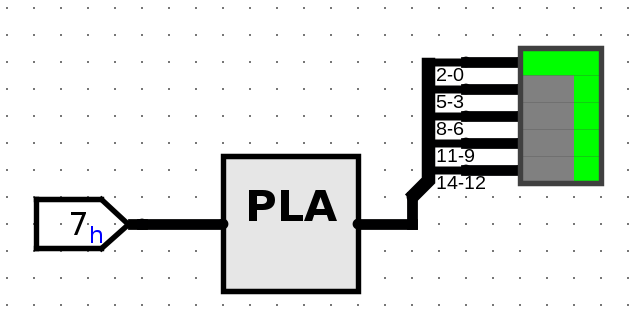
\includegraphics[width=6cm]{LEDMatrix.png}
\caption{LED Matrix}
\end{figure}

\subsubsection*{a)}
Implementiere mit Logikbausteinen deiner Wahl (Gatter-Logik, PLA, ROM...) einen
Converter, welcher einen 4-Bit BCD codierten Eingang, so umwandelt, dass eine 5×3
LED Matrix die Zahl als Dezimalzahl anzeigt.
\subsubsection*{b)}
Baue nach einem Funktionstest des Converters die Digitaluhr von einem der vorherigen 
Labore mit
den LED-Matrix Displays nach (eine 5×3 LED Matrix soll eine 7 Segment Anzeige
ersetzen).

\newpage


\end{document}
%%% Local Variables:
